\documentclass[10pt]{article}
\usepackage[margin=2cm]{geometry}
\usepackage{amsmath,amssymb}
\usepackage{booktabs}
\usepackage{graphicx}
\usepackage{float}
\usepackage{array,tabularx}
\usepackage[font=small,labelfont=bf]{caption}
\usepackage[compact]{titlesec}
\usepackage{enumitem}
\usepackage{microtype}
\usepackage[hidelinks]{hyperref}
\setlist{itemsep=1pt,topsep=3pt}
\setlength{\parskip}{4pt}
\setlength{\parindent}{0pt}
\graphicspath{{figures/}}
\newcommand{\fig}[1]{Figure~\ref{#1}}
\newcommand{\tab}[1]{Table~\ref{#1}}

\begin{document}
\sloppy

\begin{center}
{\LARGE SuperMimic on Kangaroo, M5: the 24\,h \texttt{full} and \texttt{dev} runs}\\[4pt]
The paper's algorithm with the M4 stability fixes, on all 124,077 BONES-SEED motions and on a 2.5\,h subset,
one A100 each. Branch \texttt{omm/supermimic} of pal\_mjlab, 27 October 2026.
\end{center}

\section*{Summary}

\begin{itemize}
  \item \textbf{Both runs trained without a collapse of their own.} \texttt{full}'s first job went NaN at
  17.5\,h because the simulator's constraint buffer overflowed (D44); resumed with a larger buffer, it ran
  24\,h more with no overflow. Its only other incident is a 1,400-iteration dip at 82,700, from which it
  recovered by itself.
  \item \textbf{On \texttt{dev}'s own clips, \texttt{dev} is the best policy:} 0 failed clips of 1,294 and
  tracking return 0.906 at 70,000 iterations, above every earlier result (PPO-Sim 0.770, the stability
  runs' best 0.894). \texttt{full} keeps improving slowly on those clips, to 0.894 with 0 failures at 110,000.
  \item \textbf{On motions \texttt{dev} never saw, \texttt{full} is the better policy.} On a second 2.5\,h
  sample of the library, \texttt{dev}'s final policy fails 23 of 1,242 clips (0.851); every \texttt{full}
  checkpoint fails 1 (0.862--0.878). One \texttt{full} policy handles the whole library about as well as
  \texttt{dev} handles its own 2.5\,h.
  \item \textbf{The last checkpoint is not the best.} \texttt{full}'s last checkpoint (121,000) scores 0.874
  with 3 failures, against 0.889 with none at 120,000. Both jobs end with the learning rate still at
  54--82\% of its start (the paper decays it over 250,000 iterations), so consecutive checkpoints still move
  around.
  \item \textbf{The dip followed the sampler onto physically impossible references.} Before it, four
  kneeling clips, whose retargeted knee is 17.7\,cm inside the floor in every frame, held 14\% of all
  starts. Such clips can never be tracked, so the hard sampler keeps feeding them. Since then: a dataset QA
  rule drops clips with any collision shape more than 5\,cm below the floor, and the 7-DoF data is being
  re-retargeted with the GMR fixes of the 5-DoF set (D47).
\end{itemize}

\section{The runs}

Both jobs ran the same commit on one A100 each: the paper's settings (TF32, replay 1000), compiled
imagination (D37), and the stability defaults of M4 (D39: the failure head on the rule's two errors and the
survival-weighted critic loss), on the reviewed dataset (D40).

\begin{table}[H]
\centering\small
\begin{tabularx}{\textwidth}{@{}l l >{\raggedright\arraybackslash}X >{\raggedright\arraybackslash}X@{}}\toprule
run & job & data & result \\\midrule
\texttt{dev-24h} & 62300428, \texttt{e6f3893} & \texttt{dev}: 1,294 clips, 2.55\,h & finished: 71,910 iterations in 24\,h \\
\texttt{full-24h} & 62300423, \texttt{e6f3893} & \texttt{full}: 124,077 clips, 250.9\,h & NaN at 44,620 (17.5\,h); cancelled \\
\texttt{full-24h}, resumed & 62362613, \texttt{bc44e76} & \texttt{full}, from \texttt{model\_44000}, \texttt{njmax} 1024 & finished: 121,870 iterations, 1.11\,s each \\
\bottomrule
\end{tabularx}
\end{table}

\texttt{full} trained about 40\,h in all: 15.9\,h up to iteration 44,000 in its first job, then 24\,h
resumed. ONNX policies for the robot (D48) are exported for \texttt{dev} 71,000 and \texttt{full} 121,000,
and both run in the dashboards.

\section{Benchmark on \texttt{dev}}

Every checkpoint at a multiple of 2000 (and \texttt{full}'s last) plays every clip of the reviewed
1,294-clip \texttt{dev} once from its first frame (paper F.1). \texttt{full} is drawn as one curve: its first
job up to 44,000, then the resumed job.

\begin{figure}[H]
\centering
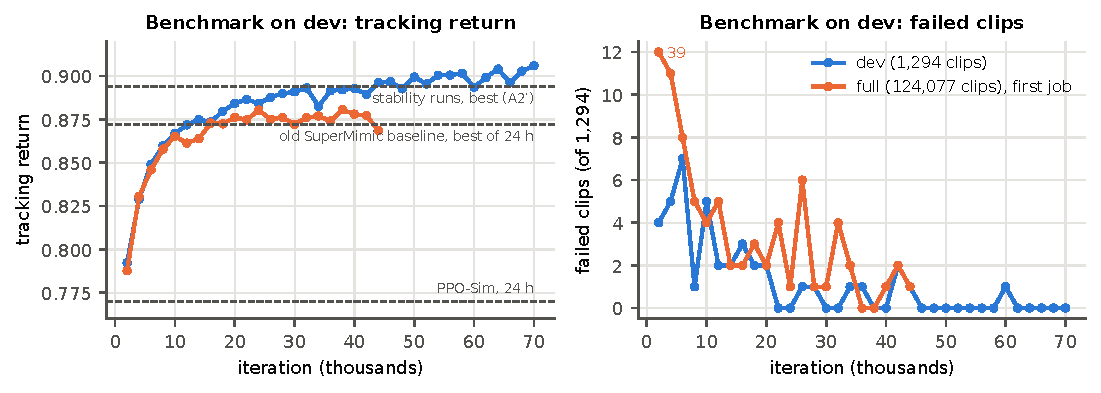
\includegraphics[width=\textwidth]{benchmark_dev.pdf}
\caption{Benchmark on \texttt{dev}. Dashed lines: earlier results on the 1,296-clip \texttt{dev} (it also
holds the two clips removed in D40, which every policy fails). Dotted: \texttt{full} resumed from 44,000.
Points outside an axis are marked at its edge with their value (84,000: inside the dip).}
\label{fig:bench}
\end{figure}

\begin{table}[H]
\centering\small
\caption{Selected checkpoints on \texttt{dev}. Body error: root-relative mean position error per body group.}
\label{tab:bench}
\begin{tabular}{@{}lrrl@{}}\toprule
checkpoint & failed clips & tracking return & body error arms / legs / torso \\\midrule
\texttt{dev}, 22,000 (7.4\,h) & 0 & 0.887 & 5.9 / 4.0 / 1.7\,cm \\
\texttt{dev}, \textbf{70,000} (23.6\,h, best) & \textbf{0} & \textbf{0.906} & 5.4 / 3.6 / 1.4\,cm \\
\texttt{dev}, 71,000 (last) & 1 & 0.904 & 5.6 / 3.6 / 1.4\,cm \\
\texttt{full}, 44,000 (resumed from here) & 1 & 0.869 & 6.1 / 4.2 / 1.6\,cm \\
\texttt{full}, 84,000 (inside the dip) & 721 & 0.389 & 23.7 / 11.5 / 5.1\,cm \\
\texttt{full}, \textbf{110,000} (best) & \textbf{0} & \textbf{0.894} & 5.5 / 3.8 / 1.3\,cm \\
\texttt{full}, 120,000 & 0 & 0.889 & 5.5 / 4.2 / 1.4\,cm \\
\texttt{full}, 121,000 (last) & 3 & 0.874 & 5.6 / 3.5 / 1.4\,cm \\\midrule
PPO-Sim, 24\,h (M4, 1,296 clips) & 15 & 0.770 & 10.7\,cm arms \\
old SuperMimic baseline, best of 24\,h (M4, 1,296 clips) & 2 & 0.872 & 6.2\,cm arms \\
stability runs, best (M4, 1,296 clips) & 2 & 0.894 & \\
\bottomrule
\end{tabular}
\end{table}

\begin{itemize}
  \item \textbf{\texttt{dev} kept improving for its whole 24\,h:} no failed clip from 46,000 on (one
  checkpoint with 1), from 0.887 at 22,000 to 0.906 at 70,000.
  \item \textbf{\texttt{full} improves slowly after the resume:} 0.877 at 46,000, 0.885--0.888 at
  70,000--82,000, 0.887--0.894 from 98,000 on, with 0--3 failures. It stays below \texttt{dev} on these clips:
  \texttt{dev} trains on each of them about 100 times as often.
  \item \textbf{The 84,000 checkpoint fell inside the dip} (721 failures); 86,000 is back at 0 failures.
\end{itemize}

\section{Motions \texttt{dev} never saw}

A second draw with the \texttt{dev} recipe (2.5\,h stratified by category, seed 1): 1,242 clips, 14 of them
also in \texttt{dev}, all of them in \texttt{full}'s training data.

\begin{figure}[H]
\centering
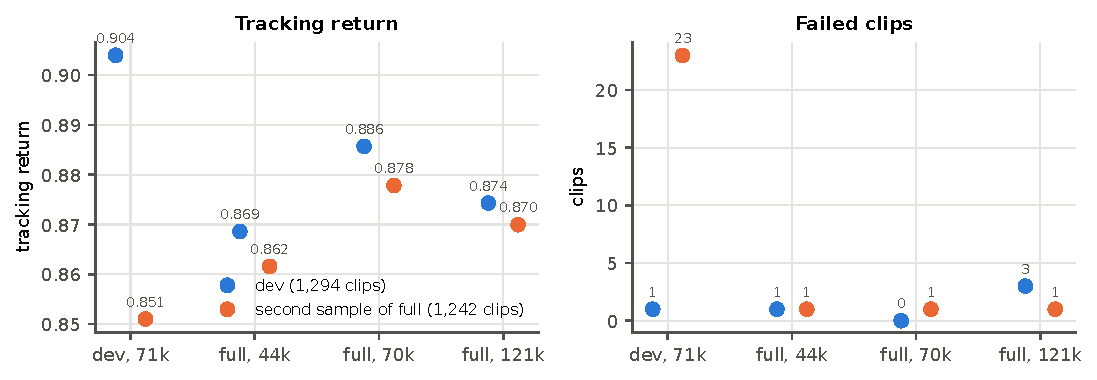
\includegraphics[width=\textwidth]{heldout.pdf}
\caption{The final policies on \texttt{dev} (blue) and on the second sample (orange).}
\label{fig:heldout}
\end{figure}

\begin{table}[H]
\centering\small
\caption{Failed clips and tracking return on both samples; body error on the second sample.}
\label{tab:heldout}
\begin{tabular}{@{}llll@{}}\toprule
policy & on \texttt{dev} (1,294 clips) & on the second sample (1,242 clips) & body error arms / legs / torso \\\midrule
\texttt{dev}, 71,000 & 1, 0.904 & 23, 0.851 & 6.8 / 4.3 / 1.7\,cm \\
\texttt{full}, 44,000 & 1, 0.869 & 1, 0.862 & 6.3 / 4.3 / 1.6\,cm \\
\texttt{full}, 70,000 & 0, 0.886 & 1, 0.878 & 5.7 / 3.9 / 1.4\,cm \\
\texttt{full}, 121,000 & 3, 0.874 & 1, 0.870 & 5.7 / 3.5 / 1.4\,cm \\
\bottomrule
\end{tabular}
\end{table}

\begin{itemize}
  \item \textbf{\texttt{dev} does not transfer to new motions:} 23 failures (1.9\%) and 0.851 on motions it
  never trained on.
  \item \textbf{\texttt{full} scores the same on both samples}, within 0.01, and fails 1 clip at every
  checkpoint: it has trained on all of them.
  \item The 250.9\,h of \texttt{full} buy coverage, not a better score on a small set.
\end{itemize}

\section{Training signals}

\begin{figure}[H]
\centering
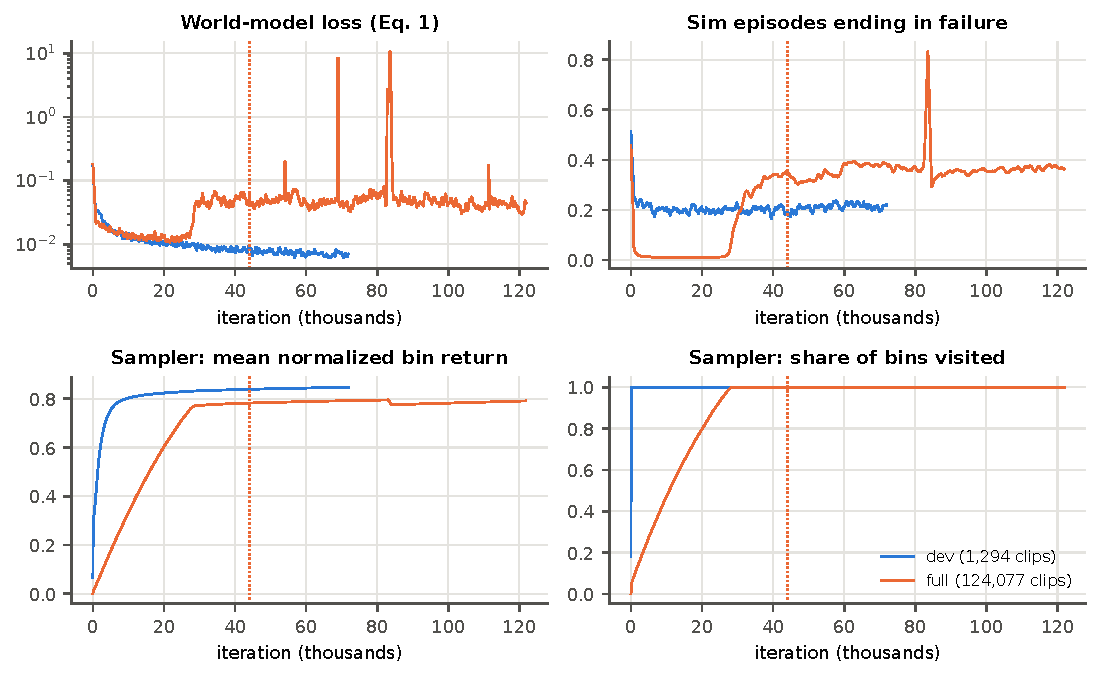
\includegraphics[width=\textwidth]{training.pdf}
\caption{TensorBoard signals. World-model loss and the share of failing episodes are moving averages. The
sampler's mean return is over all bins, unvisited ones counting as 0.}
\label{fig:training}
\end{figure}

\begin{itemize}
  \item \textbf{\texttt{full}'s sampler had visited all of its 964,607 bins by about 29,000} iterations.
  From then on, half of its starts go to the hardest 1\% of bins (by design: 40\% softmax($-25G$) and 10\%
  past weight). So its training failure rose from 1\% to 34--39\%, and its world-model loss from 0.013 to
  about 0.045. Neither is a regression: the mean normalized bin return kept rising, 0.766 at 28,000, 0.783
  at 44,000, 0.796 at 82,000, and 0.791 at the end (after the dip). Training return is not a progress
  measure on \texttt{full}; the mean bin return and the benchmark are.
  \item \textbf{\texttt{dev}:} training failure flat at 21--22\% (its sampler always has the hardest clips at
  hand), world-model loss 0.010 $\to$ 0.007, mean bin return 0.80 $\to$ 0.85.
  \item \textbf{Stability:} imagined and simulated 32-step returns correlate at $\geq 0.998$ over the last
  5,000 iterations of both runs. \texttt{dev}'s critic loss stays below 0.015 after 3,000 iterations.
  \texttt{full} had one critic-loss burst (297, in the dip) and world-model loss spikes above 0.15 at
  30,500, 41,500, 46,500, 53,500, 68,500, 81,500--84,000 and 111,000.
  \item \textbf{Memory:} 33.4\,GB (\texttt{full}), 19.6\,GB (\texttt{dev}).
\end{itemize}

\section{Two incidents on \texttt{full}}

\subsection*{The NaN at 17.5\,h: the constraint buffer (D44)}

At iteration 44,620 the world model, critic and actor went NaN within 10 iterations. All run long, MuJoCo Warp
had warned ``nefc overflow'' about 250 times per 100 iterations (up to 636 constraint rows requested, 300
allowed): dropped rows give wrong contact physics, and one non-finite state in the replay poisons every
network. \texttt{dev} warned 263 times in 24\,h. With \texttt{njmax} 1024 the resumed job never overflowed.
The training logger skips NaN values, so the collapse showed as missing losses and a jump of training
failure to 96\%.

\subsection*{The dip at 82,700: impossible references in the hard bins}

\begin{itemize}
  \item \textbf{What happened:} the world-model loss spiked first, then the policy: training failure 79\%,
  critic loss 297, imagined-vs-simulated correlation below 0.9. By 84,100 it had recovered by itself.
  \item \textbf{Where the sampler had put its starts} (its state is in every checkpoint): at 80,000--82,000,
  four clips held about 14\% of all starts, \texttt{kneeling\_loop\_102/103\_\_A064} and their mirrors
  (3.3--3.8\% each). After the dip the hard bins spread out (top clip 0.7\%), then
  \texttt{crossed\_legs\_R\_001\_\_A428}--\texttt{A432} took the top places (3--4\% each).
  \item \textbf{Those clips are physically impossible in the 7-DoF data} (pal\_mjlab's collision model): in
  \texttt{kneeling\_loop} the right knee is 17.4--17.7\,cm in the floor in every frame; in
  \texttt{crossed\_legs} the legs pass 9--14\,cm through each other and arms and grippers go 16--73\,cm into
  the floor. They had all passed the dataset QA, which checks link origins only (paper E: $-12$\,cm once,
  $-8$\,cm sustained).
  \item \textbf{Likely mechanism (one occurrence):} a bin that can never be tracked never earns its return,
  so the hard sampler keeps feeding it. The replay fills with failing, contact-rich data from a handful of
  motions; the world model's fit degrades there, and the policy follows the wrong model.
  \item \textbf{Consequences} (user, 27 October): the dataset QA now drops clips with any collision shape
  more than 5\,cm below the floor, and the 7-DoF data is re-retargeted with the 5-DoF set's GMR fixes:
  self-collision avoidance, the clip's own floor, the torso weight, GMR's IK limits, and pal\_mjlab's
  grippers with a physically paired wrist target (D47). In the current 7-DoF data, 30.6\% of frames have a
  self-penetration over 1\,cm and 28\% a foot over 1\,cm in the floor (1,000 random clips).
\end{itemize}

\section{The last checkpoint is not the best}

\begin{itemize}
  \item \texttt{full} 121,000 is worse than 120,000 on most clips (per clip, median $-0.007$; 63\% of clips
  worse) and fails 3, where 120,000 fails none. Consecutive checkpoints usually differ by $\pm$0.003--0.005
  per clip. On the second sample, 121,000 (0.870) is also below 70,000 (0.878). \texttt{dev}'s last
  checkpoint (71,000: 1 failure, 0.904) is also just below its best (70,000: 0, 0.906).
  \item \textbf{The learning rate is still high when the jobs end.} The paper's cosine schedule decays to
  3\% over 250,000 iterations; \texttt{full} stops at 121,870 with the rate at 54\% of its start,
  \texttt{dev} at 71,910 with 82\%. So checkpoints keep moving, and the last one is a sample of that noise.
  \item \textbf{To make the last checkpoint the best:} decay the learning rate over the run's own length,
  or keep an average of the policy weights. Not done yet.
\end{itemize}

\section{Caveats}

\begin{itemize}
  \item One seed per run.
  \item The benchmark runs with \texttt{njmax} 1024; \texttt{dev} and \texttt{full}'s first job trained with
  300, so their contacts are simulated more exactly here than in training.
  \item A checkpoint takes 5.2\,min on the local GPU, about 4$\times$ the M4 benchmarks; the larger constraint
  buffer is the likely cause (not measured).
\end{itemize}

\section{Decisions and next steps}

\begin{itemize}
  \item \textbf{D44:} \texttt{njmax} 1024. \textbf{D48:} ONNX policies at every checkpoint, and a script for
  older ones. \textbf{D47} (running): the 7-DoF data re-retargeted and re-QA'd with the floor rule; it
  replaces the current set, which is archived.
  \item \textbf{Next:}
  \begin{itemize}
    \item a \texttt{full} run on the new 7-DoF data, benchmarked on a sample of it;
    \item a learning-rate schedule fitted to the run length, or a weight average, so the last checkpoint
    is the best (needs the user's go);
    \item the 5-DoF \texttt{full} run (job 62432587) is queued on Leonardo;
    \item option: an upper-body goal interface on a frozen checkpoint (paper Appendix B).
  \end{itemize}
\end{itemize}

\appendix
\section{Reproduction}

\begin{footnotesize}
\begin{verbatim}
# runs (Leonardo, lazyhpc run folders 20261026-015332_{SMfull,SMdev}_e6f3893, 20261026-192504_SMfull2_bc44e76)
python -m pal_mjlab.scripts.supermimic.train Mjlab-SuperMimic-Flat-Pal-Kangaroo-Grippers-ArmWaist1Hz \
  --library <dataset>/libraries/{full,dev} --agent.experiment-name supermimic_d39 --agent.run-name {full,dev}-24h
# benchmark: dev, and the second sample (bones_to_library --subset dev --seed 1)
python -m pal_mjlab.scripts.supermimic.eval --task <task> --library <library> \
  --checkpoints <run>/model_*.pt --out-dir logs/supermimic_eval/m5_<name>
# ONNX for older checkpoints (D48)
python -m pal_mjlab.scripts.supermimic.export_onnx <task> --library <library> <run>/model_N.pt
# figures and this report
python docs/supermimic/m5/make_figures.py && (cd docs/supermimic/m5 && latexmk -pdf report.tex)
\end{verbatim}
\end{footnotesize}

\end{document}
